% Options for packages loaded elsewhere
\PassOptionsToPackage{unicode}{hyperref}
\PassOptionsToPackage{hyphens}{url}
\documentclass[
]{article}
\usepackage{xcolor}
\usepackage[margin=1in]{geometry}
\usepackage{amsmath,amssymb}
\setcounter{secnumdepth}{5}
\usepackage{iftex}
\ifPDFTeX
  \usepackage[T1]{fontenc}
  \usepackage[utf8]{inputenc}
  \usepackage{textcomp} % provide euro and other symbols
\else % if luatex or xetex
  \usepackage{unicode-math} % this also loads fontspec
  \defaultfontfeatures{Scale=MatchLowercase}
  \defaultfontfeatures[\rmfamily]{Ligatures=TeX,Scale=1}
\fi
\usepackage{lmodern}
\ifPDFTeX\else
  % xetex/luatex font selection
\fi
% Use upquote if available, for straight quotes in verbatim environments
\IfFileExists{upquote.sty}{\usepackage{upquote}}{}
\IfFileExists{microtype.sty}{% use microtype if available
  \usepackage[]{microtype}
  \UseMicrotypeSet[protrusion]{basicmath} % disable protrusion for tt fonts
}{}
\makeatletter
\@ifundefined{KOMAClassName}{% if non-KOMA class
  \IfFileExists{parskip.sty}{%
    \usepackage{parskip}
  }{% else
    \setlength{\parindent}{0pt}
    \setlength{\parskip}{6pt plus 2pt minus 1pt}}
}{% if KOMA class
  \KOMAoptions{parskip=half}}
\makeatother
\usepackage{color}
\usepackage{fancyvrb}
\newcommand{\VerbBar}{|}
\newcommand{\VERB}{\Verb[commandchars=\\\{\}]}
\DefineVerbatimEnvironment{Highlighting}{Verbatim}{commandchars=\\\{\}}
% Add ',fontsize=\small' for more characters per line
\usepackage{framed}
\definecolor{shadecolor}{RGB}{248,248,248}
\newenvironment{Shaded}{\begin{snugshade}}{\end{snugshade}}
\newcommand{\AlertTok}[1]{\textcolor[rgb]{0.94,0.16,0.16}{#1}}
\newcommand{\AnnotationTok}[1]{\textcolor[rgb]{0.56,0.35,0.01}{\textbf{\textit{#1}}}}
\newcommand{\AttributeTok}[1]{\textcolor[rgb]{0.13,0.29,0.53}{#1}}
\newcommand{\BaseNTok}[1]{\textcolor[rgb]{0.00,0.00,0.81}{#1}}
\newcommand{\BuiltInTok}[1]{#1}
\newcommand{\CharTok}[1]{\textcolor[rgb]{0.31,0.60,0.02}{#1}}
\newcommand{\CommentTok}[1]{\textcolor[rgb]{0.56,0.35,0.01}{\textit{#1}}}
\newcommand{\CommentVarTok}[1]{\textcolor[rgb]{0.56,0.35,0.01}{\textbf{\textit{#1}}}}
\newcommand{\ConstantTok}[1]{\textcolor[rgb]{0.56,0.35,0.01}{#1}}
\newcommand{\ControlFlowTok}[1]{\textcolor[rgb]{0.13,0.29,0.53}{\textbf{#1}}}
\newcommand{\DataTypeTok}[1]{\textcolor[rgb]{0.13,0.29,0.53}{#1}}
\newcommand{\DecValTok}[1]{\textcolor[rgb]{0.00,0.00,0.81}{#1}}
\newcommand{\DocumentationTok}[1]{\textcolor[rgb]{0.56,0.35,0.01}{\textbf{\textit{#1}}}}
\newcommand{\ErrorTok}[1]{\textcolor[rgb]{0.64,0.00,0.00}{\textbf{#1}}}
\newcommand{\ExtensionTok}[1]{#1}
\newcommand{\FloatTok}[1]{\textcolor[rgb]{0.00,0.00,0.81}{#1}}
\newcommand{\FunctionTok}[1]{\textcolor[rgb]{0.13,0.29,0.53}{\textbf{#1}}}
\newcommand{\ImportTok}[1]{#1}
\newcommand{\InformationTok}[1]{\textcolor[rgb]{0.56,0.35,0.01}{\textbf{\textit{#1}}}}
\newcommand{\KeywordTok}[1]{\textcolor[rgb]{0.13,0.29,0.53}{\textbf{#1}}}
\newcommand{\NormalTok}[1]{#1}
\newcommand{\OperatorTok}[1]{\textcolor[rgb]{0.81,0.36,0.00}{\textbf{#1}}}
\newcommand{\OtherTok}[1]{\textcolor[rgb]{0.56,0.35,0.01}{#1}}
\newcommand{\PreprocessorTok}[1]{\textcolor[rgb]{0.56,0.35,0.01}{\textit{#1}}}
\newcommand{\RegionMarkerTok}[1]{#1}
\newcommand{\SpecialCharTok}[1]{\textcolor[rgb]{0.81,0.36,0.00}{\textbf{#1}}}
\newcommand{\SpecialStringTok}[1]{\textcolor[rgb]{0.31,0.60,0.02}{#1}}
\newcommand{\StringTok}[1]{\textcolor[rgb]{0.31,0.60,0.02}{#1}}
\newcommand{\VariableTok}[1]{\textcolor[rgb]{0.00,0.00,0.00}{#1}}
\newcommand{\VerbatimStringTok}[1]{\textcolor[rgb]{0.31,0.60,0.02}{#1}}
\newcommand{\WarningTok}[1]{\textcolor[rgb]{0.56,0.35,0.01}{\textbf{\textit{#1}}}}
\usepackage{longtable,booktabs,array}
\newcounter{none} % for unnumbered tables
\usepackage{calc} % for calculating minipage widths
% Correct order of tables after \paragraph or \subparagraph
\usepackage{etoolbox}
\makeatletter
\patchcmd\longtable{\par}{\if@noskipsec\mbox{}\fi\par}{}{}
\makeatother
% Allow footnotes in longtable head/foot
\IfFileExists{footnotehyper.sty}{\usepackage{footnotehyper}}{\usepackage{footnote}}
\makesavenoteenv{longtable}
\usepackage{graphicx}
\makeatletter
\newsavebox\pandoc@box
\newcommand*\pandocbounded[1]{% scales image to fit in text height/width
  \sbox\pandoc@box{#1}%
  \Gscale@div\@tempa{\textheight}{\dimexpr\ht\pandoc@box+\dp\pandoc@box\relax}%
  \Gscale@div\@tempb{\linewidth}{\wd\pandoc@box}%
  \ifdim\@tempb\p@<\@tempa\p@\let\@tempa\@tempb\fi% select the smaller of both
  \ifdim\@tempa\p@<\p@\scalebox{\@tempa}{\usebox\pandoc@box}%
  \else\usebox{\pandoc@box}%
  \fi%
}
% Set default figure placement to htbp
\def\fps@figure{htbp}
\makeatother
\setlength{\emergencystretch}{3em} % prevent overfull lines
\providecommand{\tightlist}{%
  \setlength{\itemsep}{0pt}\setlength{\parskip}{0pt}}
\usepackage{booktabs}
\usepackage{caption}
\usepackage{longtable}
\usepackage{colortbl}
\usepackage{array}
\usepackage{anyfontsize}
\usepackage{multirow}
\usepackage{bookmark}
\IfFileExists{xurl.sty}{\usepackage{xurl}}{} % add URL line breaks if available
\urlstyle{same}
\hypersetup{
  pdftitle={IndepAssoc: Confounder-Adjusted Association Testing via Propensity Score Methods},
  pdfauthor={Mostafa Elshamy},
  hidelinks,
  pdfcreator={LaTeX via pandoc}}

\title{IndepAssoc: Confounder-Adjusted Association Testing via
Propensity Score Methods}
\author{Mostafa Elshamy}
\date{2026-07-25}

\begin{document}
\maketitle

{
\setcounter{tocdepth}{3}
\tableofcontents
}
\section{Introduction}\label{introduction}

\texttt{IndepAssoc} generalizes the propensity-score-based analysis
pipeline used in retrospective cohort studies to answer the core
scientific question:

\begin{quote}
\emph{Is a risk factor or exposure independently associated with an
outcome, after adjusting for confounders?}
\end{quote}

Matching is used in the context of estimating the effect of a binary
treatment or exposure on an outcome while controlling for measured
pre-treatment variables. The goal of matching is to produce
\textbf{covariate balance}, i.e., for the distributions of covariates in
the two groups to be approximately equal, as they would be in a
successful randomized experiment.

A matching analysis with \texttt{IndepAssoc} involves four primary
steps:

\begin{enumerate}
\def\labelenumi{\arabic{enumi}.}
\tightlist
\item
  Building a propensity score model
\item
  Matching cohorts
\item
  Assessing covariate balance
\item
  Estimating the treatment effect using multiple regression approaches
\end{enumerate}

\begin{Shaded}
\begin{Highlighting}[]
\FunctionTok{library}\NormalTok{(IndepAssoc)}

\NormalTok{data }\OtherTok{\textless{}{-}} \FunctionTok{read.csv}\NormalTok{(}\FunctionTok{system.file}\NormalTok{(}\StringTok{"extdata/sample\_psm\_dataset.csv"}\NormalTok{, }\AttributeTok{package =} \StringTok{"IndepAssoc"}\NormalTok{))}
\FunctionTok{head}\NormalTok{(data, }\DecValTok{5}\NormalTok{)}
\CommentTok{\#\textgreater{}   treatment age      bmi smoker hypertension numeric\_outcome binary\_outcome}
\CommentTok{\#\textgreater{} 1         0  43 28.43064      0            0        2.087897              0}
\CommentTok{\#\textgreater{} 2         1  52 24.36025      1            0        8.912335              0}
\CommentTok{\#\textgreater{} 3         1  52 24.92394      0            0        4.368925              1}
\CommentTok{\#\textgreater{} 4         1  42 20.98988      1            0        3.306441              0}
\CommentTok{\#\textgreater{} 5         0  68 24.92595      0            1        1.563577              0}
\end{Highlighting}
\end{Shaded}

\newpage

\section{Propensity Score Model}\label{propensity-score-model}

The first step is to estimate a propensity score for each unit---the
predicted probability of receiving treatment given the covariates,
estimated via logistic regression.

\begin{Shaded}
\begin{Highlighting}[]
\NormalTok{ps }\OtherTok{\textless{}{-}} \FunctionTok{build\_ps\_model}\NormalTok{(}
  \AttributeTok{data =}\NormalTok{ data,}
  \AttributeTok{exposure =} \StringTok{"treatment"}\NormalTok{,}
  \AttributeTok{covariates =} \FunctionTok{c}\NormalTok{(}\StringTok{"age"}\NormalTok{, }\StringTok{"bmi"}\NormalTok{, }\StringTok{"smoker"}\NormalTok{, }\StringTok{"hypertension"}\NormalTok{)}
\NormalTok{)}

\NormalTok{knitr}\SpecialCharTok{::}\FunctionTok{kable}\NormalTok{(}
  \FunctionTok{summary}\NormalTok{(ps}\SpecialCharTok{$}\NormalTok{model)}\SpecialCharTok{$}\NormalTok{coefficients,}
  \AttributeTok{caption =} \StringTok{"Propensity score model coefficients"}\NormalTok{,}
  \AttributeTok{digits =} \DecValTok{4}
\NormalTok{)}
\end{Highlighting}
\end{Shaded}

\begin{longtable}[]{@{}lrrrr@{}}
\caption{Propensity score model coefficients}\tabularnewline
\toprule\noalign{}
& Estimate & Std. Error & z value &
Pr(\textgreater\textbar z\textbar) \\
\midrule\noalign{}
\endfirsthead
\toprule\noalign{}
& Estimate & Std. Error & z value &
Pr(\textgreater\textbar z\textbar) \\
\midrule\noalign{}
\endhead
\bottomrule\noalign{}
\endlastfoot
(Intercept) & -0.2840 & 1.1960 & -0.2374 & 0.8123 \\
age & 0.0063 & 0.0148 & 0.4249 & 0.6709 \\
bmi & -0.0039 & 0.0356 & -0.1094 & 0.9129 \\
smoker & 0.4143 & 0.3172 & 1.3059 & 0.1916 \\
hypertension & -0.2234 & 0.2925 & -0.7638 & 0.4450 \\
\end{longtable}

\newpage

\section{Matching}\label{matching}

We perform 1:1 nearest-neighbor matching on the propensity score without
replacement, with a caliper of 0.2 standard deviations of the logit(PS).

\begin{Shaded}
\begin{Highlighting}[]
\NormalTok{matched }\OtherTok{\textless{}{-}} \FunctionTok{match\_cohort}\NormalTok{(ps, }\AttributeTok{caliper =} \FloatTok{0.2}\NormalTok{)}
\FunctionTok{cat}\NormalTok{(}\StringTok{"Unmatched:"}\NormalTok{, }\FunctionTok{nrow}\NormalTok{(data), }\StringTok{"{-}\textgreater{} Matched:"}\NormalTok{, }\FunctionTok{nrow}\NormalTok{(matched}\SpecialCharTok{$}\NormalTok{data), }\StringTok{"observations}\SpecialCharTok{\textbackslash{}n}\StringTok{"}\NormalTok{)}
\CommentTok{\#\textgreater{} Unmatched: 200 {-}\textgreater{} Matched: 186 observations}
\end{Highlighting}
\end{Shaded}

\newpage

\section{Covariate Balance}\label{covariate-balance}

\begin{Shaded}
\begin{Highlighting}[]
\NormalTok{balance }\OtherTok{\textless{}{-}} \FunctionTok{check\_balance}\NormalTok{(matched, }\AttributeTok{threshold =} \FloatTok{0.10}\NormalTok{)}
\FunctionTok{cat}\NormalTok{(}\StringTok{"All balanced:"}\NormalTok{, balance}\SpecialCharTok{$}\NormalTok{all\_balanced, }\StringTok{"}\SpecialCharTok{\textbackslash{}n}\StringTok{"}\NormalTok{)}
\CommentTok{\#\textgreater{} All balanced: TRUE}
\end{Highlighting}
\end{Shaded}

\subsection{Love Plot}\label{love-plot}

\begin{Shaded}
\begin{Highlighting}[]
\FunctionTok{plot\_love}\NormalTok{(matched, }\AttributeTok{threshold =} \FloatTok{0.10}\NormalTok{)}
\end{Highlighting}
\end{Shaded}

\begin{figure}
\centering
\pandocbounded{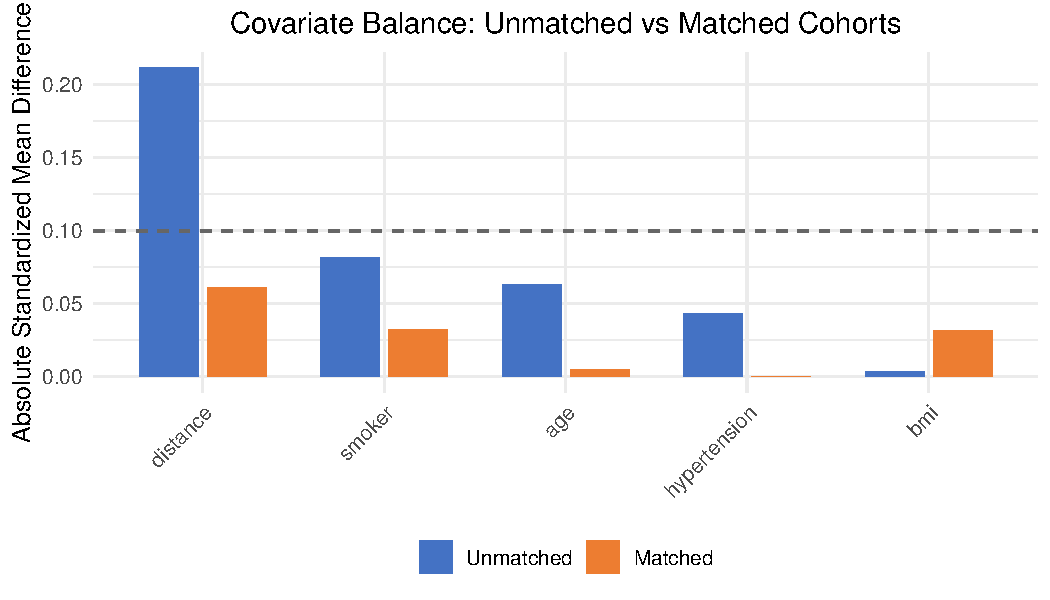
\includegraphics[keepaspectratio,alt={Love plot: ASMD before and after matching.}]{IndepAssoc-pdf_files/IndepAssoc-pdf_files/figure-latex/love-plot-1.pdf}}
\caption{Love plot: ASMD before and after matching.}
\end{figure}

\newpage

\section{Descriptive Tables}\label{descriptive-tables}

\subsection{Unmatched Data}\label{unmatched-data}

\begin{Shaded}
\begin{Highlighting}[]
\FunctionTok{table\_unmatched}\NormalTok{(data, }\StringTok{"treatment"}\NormalTok{, }\FunctionTok{c}\NormalTok{(}\StringTok{"age"}\NormalTok{, }\StringTok{"bmi"}\NormalTok{, }\StringTok{"smoker"}\NormalTok{, }\StringTok{"hypertension"}\NormalTok{))}
\end{Highlighting}
\end{Shaded}

\begin{table}[t]
\fontsize{12.0pt}{14.0pt}\selectfont
\begin{tabular*}{\linewidth}{@{\extracolsep{\fill}}lccc}
\toprule
\textbf{Characteristic} & \textbf{0}  N = 102\textsuperscript{\textit{1}} & \textbf{1}  N = 98\textsuperscript{\textit{1}} & \textbf{p-value}\textsuperscript{\textit{2}} \\ 
\midrule\addlinespace[2.5pt]
age & 51.0 (42.0, 56.0) & 50.0 (44.0, 57.0) & 0.5 \\ 
bmi & 24.8 (21.6, 27.3) & 24.7 (21.8, 27.5) & >0.9 \\ 
smoker & 25 (25\%) & 32 (33\%) & 0.3 \\ 
hypertension & 45 (44\%) & 39 (40\%) & 0.6 \\ 
\bottomrule
\end{tabular*}
\begin{minipage}{\linewidth}
\vspace{.05em}
\textsuperscript{\textit{1}}Median (Q1, Q3); n (\%)\\
\textsuperscript{\textit{2}}Wilcoxon rank sum test; Pearson's Chi-squared test\\
\end{minipage}
\end{table}

\subsection{Matched Data}\label{matched-data}

\begin{Shaded}
\begin{Highlighting}[]
\FunctionTok{table\_matched}\NormalTok{(matched, }\FunctionTok{c}\NormalTok{(}\StringTok{"age"}\NormalTok{, }\StringTok{"bmi"}\NormalTok{, }\StringTok{"smoker"}\NormalTok{, }\StringTok{"hypertension"}\NormalTok{))}
\end{Highlighting}
\end{Shaded}

\begin{table}[t]
\fontsize{12.0pt}{14.0pt}\selectfont
\begin{tabular*}{\linewidth}{@{\extracolsep{\fill}}lcccccc}
\toprule
 & \multicolumn{3}{c}{{\textbf{Table 1}}} & \multicolumn{3}{c}{{\textbf{Table 2}}} \\ 
\cmidrule(lr){2-4} \cmidrule(lr){5-7}
\textbf{Characteristic} & \textbf{0}  N = 93\textsuperscript{\textit{1}} & \textbf{1}  N = 93\textsuperscript{\textit{1}} & \textbf{p-value}\textsuperscript{\textit{2}} & \textbf{0}  N = 93\textsuperscript{\textit{3}} & \textbf{1}  N = 93\textsuperscript{\textit{3}} & \textbf{p-value}\textsuperscript{\textit{4}} \\ 
\midrule\addlinespace[2.5pt]
smoker & 24 (26\%) & 27 (29\%) & 0.2 &  &  &  \\ 
hypertension & 37 (40\%) & 37 (40\%) & >0.9 &  &  &  \\ 
age &  &  &  & 51.0 (42.0, 56.0) & 50.0 (44.0, 57.0) & 0.001 \\ 
bmi &  &  &  & 25.0 (21.6, 27.3) & 24.8 (21.9, 27.5) & 0.9 \\ 
\bottomrule
\end{tabular*}
\begin{minipage}{\linewidth}
\vspace{.05em}
\textsuperscript{\textit{1}}n (\%)\\
\textsuperscript{\textit{2}}McNemar's Chi-squared test with continuity correction; McNemar's Chi-squared test\\
\textsuperscript{\textit{3}}Median (Q1, Q3)\\
\textsuperscript{\textit{4}}Wilcoxon signed rank test with continuity correction\\
\end{minipage}
\end{table}

\newpage

\section{Outcome Models}\label{outcome-models}

\subsection{Binary Outcome}\label{binary-outcome}

\begin{Shaded}
\begin{Highlighting}[]
\NormalTok{models\_bin }\OtherTok{\textless{}{-}} \FunctionTok{fit\_all\_models}\NormalTok{(}
  \AttributeTok{ps\_model =}\NormalTok{ ps,}
  \AttributeTok{matched\_data =}\NormalTok{ matched}\SpecialCharTok{$}\NormalTok{data,}
  \AttributeTok{outcome =} \StringTok{"binary\_outcome"}\NormalTok{,}
  \AttributeTok{type =} \StringTok{"binary"}
\NormalTok{)}

\NormalTok{knitr}\SpecialCharTok{::}\FunctionTok{kable}\NormalTok{(models\_bin}\SpecialCharTok{$}\NormalTok{summary\_w, }\AttributeTok{caption =} \StringTok{"Binary outcome models"}\NormalTok{, }\AttributeTok{digits =} \DecValTok{4}\NormalTok{)}
\end{Highlighting}
\end{Shaded}

\begin{longtable}[]{@{}llrlr@{}}
\caption{Binary outcome models}\tabularnewline
\toprule\noalign{}
label & Model & OR & CI\_95 & p \\
\midrule\noalign{}
\endfirsthead
\toprule\noalign{}
label & Model & OR & CI\_95 & p \\
\midrule\noalign{}
\endhead
\bottomrule\noalign{}
\endlastfoot
binary\_outcome & Fully adjusted logistic & 2.87 & 5.48-240.96 &
0.0011 \\
binary\_outcome & Conditional logit & 2.27 & 4.16-64.16 & 0.0083 \\
binary\_outcome & Doubly robust logistic & 2.64 & 5.1-163.33 & 0.0031 \\
binary\_outcome & Mixed effect logistic & 2.37 & 4.33-75.75 & 0.0049 \\
\end{longtable}

\subsection{Continuous Outcome}\label{continuous-outcome}

\begin{Shaded}
\begin{Highlighting}[]
\NormalTok{models\_cont }\OtherTok{\textless{}{-}} \FunctionTok{fit\_all\_models}\NormalTok{(}
  \AttributeTok{ps\_model =}\NormalTok{ ps,}
  \AttributeTok{matched\_data =}\NormalTok{ matched}\SpecialCharTok{$}\NormalTok{data,}
  \AttributeTok{outcome =} \StringTok{"numeric\_outcome"}\NormalTok{,}
  \AttributeTok{type =} \StringTok{"continuous"}
\NormalTok{)}

\NormalTok{knitr}\SpecialCharTok{::}\FunctionTok{kable}\NormalTok{(models\_cont}\SpecialCharTok{$}\NormalTok{summary\_w, }\AttributeTok{caption =} \StringTok{"Continuous outcome models"}\NormalTok{, }\AttributeTok{digits =} \DecValTok{4}\NormalTok{)}
\end{Highlighting}
\end{Shaded}

\begin{longtable}[]{@{}
  >{\raggedright\arraybackslash}p{(\linewidth - 10\tabcolsep) * \real{0.1702}}
  >{\raggedright\arraybackslash}p{(\linewidth - 10\tabcolsep) * \real{0.3511}}
  >{\raggedleft\arraybackslash}p{(\linewidth - 10\tabcolsep) * \real{0.0745}}
  >{\raggedright\arraybackslash}p{(\linewidth - 10\tabcolsep) * \real{0.1489}}
  >{\raggedright\arraybackslash}p{(\linewidth - 10\tabcolsep) * \real{0.2234}}
  >{\raggedleft\arraybackslash}p{(\linewidth - 10\tabcolsep) * \real{0.0319}}@{}}
\caption{Continuous outcome models}\tabularnewline
\toprule\noalign{}
\begin{minipage}[b]{\linewidth}\raggedright
label
\end{minipage} & \begin{minipage}[b]{\linewidth}\raggedright
Model
\end{minipage} & \begin{minipage}[b]{\linewidth}\raggedleft
SC
\end{minipage} & \begin{minipage}[b]{\linewidth}\raggedright
CI\_95
\end{minipage} & \begin{minipage}[b]{\linewidth}\raggedright
SC\_CI\_95
\end{minipage} & \begin{minipage}[b]{\linewidth}\raggedleft
p
\end{minipage} \\
\midrule\noalign{}
\endfirsthead
\toprule\noalign{}
\begin{minipage}[b]{\linewidth}\raggedright
label
\end{minipage} & \begin{minipage}[b]{\linewidth}\raggedright
Model
\end{minipage} & \begin{minipage}[b]{\linewidth}\raggedleft
SC
\end{minipage} & \begin{minipage}[b]{\linewidth}\raggedright
CI\_95
\end{minipage} & \begin{minipage}[b]{\linewidth}\raggedright
SC\_CI\_95
\end{minipage} & \begin{minipage}[b]{\linewidth}\raggedleft
p
\end{minipage} \\
\midrule\noalign{}
\endhead
\bottomrule\noalign{}
\endlastfoot
numeric\_outcome & Fully adjusted linear regression & 0.1509 &
0.1912-0.1912 & 0.151(0.1912-0.1912) & 0 \\
numeric\_outcome & Conditional linear regression & 0.1517 & 0.201-0.201
& 0.152(0.201-0.201) & 0 \\
numeric\_outcome & Doubly robust linear regression & 0.1490 &
0.1906-0.1906 & 0.149(0.1906-0.1906) & 0 \\
numeric\_outcome & Mixed effect linear regression & 0.1517 & 0.201-0.201
& 0.152(0.201-0.201) & 0 \\
\end{longtable}

\newpage

\section{Paired Statistical Tests}\label{paired-statistical-tests}

\subsection{McNemar Test}\label{mcnemar-test}

\begin{Shaded}
\begin{Highlighting}[]
\FunctionTok{mcnemar\_test}\NormalTok{(matched}\SpecialCharTok{$}\NormalTok{data, }\StringTok{"binary\_outcome"}\NormalTok{, }\StringTok{"treatment"}\NormalTok{)}
\CommentTok{\#\textgreater{}            label   0(n=93)   1(n=93) group1 group2 statistic df          p      p.adj p.adj.signif       method}
\CommentTok{\#\textgreater{} 1 binary\_outcome 28(30.1\%) 47(50.5\%)      0      1  6.612245  1 0.01012799 0.01012799            * McNemar test}
\end{Highlighting}
\end{Shaded}

\subsection{Paired Wilcoxon Test}\label{paired-wilcoxon-test}

\begin{Shaded}
\begin{Highlighting}[]
\FunctionTok{paired\_wilcoxon\_test}\NormalTok{(matched}\SpecialCharTok{$}\NormalTok{data, }\StringTok{"numeric\_outcome"}\NormalTok{, }\StringTok{"treatment"}\NormalTok{)}
\CommentTok{\#\textgreater{}             label      0(n=93)      1(n=93)              p.value}
\CommentTok{\#\textgreater{} 1 numeric\_outcome 2.7(1.5{-}4.2) 4.9(3.4{-}6.4) 2.02367198589108e{-}07}
\end{Highlighting}
\end{Shaded}

\newpage

\section{Full Pipeline}\label{full-pipeline}

\begin{Shaded}
\begin{Highlighting}[]
\NormalTok{result }\OtherTok{\textless{}{-}} \FunctionTok{run\_pipeline}\NormalTok{(}
  \AttributeTok{data =}\NormalTok{ data,}
  \AttributeTok{exposure =} \StringTok{"treatment"}\NormalTok{,}
  \AttributeTok{covariates =} \FunctionTok{c}\NormalTok{(}\StringTok{"age"}\NormalTok{, }\StringTok{"bmi"}\NormalTok{, }\StringTok{"smoker"}\NormalTok{, }\StringTok{"hypertension"}\NormalTok{),}
  \AttributeTok{outcome =} \StringTok{"binary\_outcome"}\NormalTok{,}
  \AttributeTok{type =} \StringTok{"binary"}
\NormalTok{)}
\FunctionTok{summary}\NormalTok{(result)}
\end{Highlighting}
\end{Shaded}

\section{Exporting Results}\label{exporting-results}

\begin{Shaded}
\begin{Highlighting}[]
\FunctionTok{export\_results}\NormalTok{(result, }\AttributeTok{output\_dir =} \StringTok{"output"}\NormalTok{)}
\end{Highlighting}
\end{Shaded}

\newpage

\section{References}\label{references}

\begin{itemize}
\item
  Benedetto, U., Head, S.J., Angelini, G.D. and Blackstone, E.H. (2018).
  Statistical primer: propensity score matching and its alternatives.
  \emph{European Journal of Cardio-Thoracic Surgery}, 53(6),
  pp.1112-1117.
\item
  Ho, D.E., Imai, K., King, G. and Stuart, E.A. (2007). Matching as
  Nonparametric Preprocessing for Reducing Model Dependence in
  Parametric Causal Inference. \emph{Political Analysis}, 15(3),
  pp.199-236.
\item
  Rosenbaum, P.R. and Rubin, D.B. (1983). The Central Role of the
  Propensity Score in Observational Studies for Causal Effects.
  \emph{Biometrika}, 70(1), pp.41-55.
\item
  Stuart, E.A. (2010). Matching Methods for Causal Inference: A Review
  and a Look Forward. \emph{Statistical Science}, 25(1), pp.1-21.
\end{itemize}

\end{document}
